\documentclass[a4paper,11pt,titlepage,uplatex]{jsarticle}

% プリアンブルを外部ファイル化しておきました。中身はmacro.texで確認できます。

\usepackage[dvipdfmx]{graphicx,xcolor}% ドライバ指定
\usepackage[top=30truemm,bottom=30truemm,left=25truemm,right=25truemm]{geometry} % 余白設定

% 画像
\usepackage{here, subfig}
\usepackage{docmute} % ファイル分割用
\usepackage[cc]{titlepic}

% 数式関連
\usepackage{amsmath,amsfonts,amssymb,mathtools,amsthm}
\usepackage{bm} % ボールド体のベクトルを出力するときには\vb{a}ではなく\bm{a}としてください。\bmの方が綺麗に出力できる。
\usepackage{empheq} % 連立方程式をきれいに書いてくれる
\usepackage{physics} % 微分記号とか
\usepackage[separate-uncertainty]{siunitx} % SIUNITX

% 数式、図、表番号の変更
\makeatletter
\@addtoreset{equation}{section} % 章ごとに番号をリセット
\@addtoreset{figure}{section}
\@addtoreset{table}{section}
\def\theequation{\thesection.\arabic{equation}} % 章.何番目 と変更
\def\thefigure{\thesection.\arabic{figure}}
\def\thetable{\thesection.\arabic{table}}
\makeatother

% -------------------
% 定理環境付近
\usepackage{tcolorbox} % 色付きの囲み
\tcbuselibrary{breakable, skins, theorems}
\usepackage{ascmac} % 囲み \begin{itembox}ができる。

% ----------

\usepackage{enumitem} % enumium環境いじるために必要
\renewcommand{\labelenumi}{\theenumi.}
\renewcommand{\theenumi}{\Alph{enumi}}

% ------------ url関係
\usepackage{url}
\usepackage[dvipdfmx]{hyperref}
\hypersetup{
	 colorlinks=true,
	 citecolor=blue,
	 linkcolor=black,
	 urlcolor=blue
}
\usepackage{pxjahyper}
% ---------

% 表関連のパッケージ
\usepackage{booktabs}
\usepackage{multirow}
\usepackage{longtable}
\usepackage{arydshln}% 表で破線を使うため
\usepackage{multicol}
% longtableをusepackageする場合は順番が重要らしいです。longtableとarydshlnの順番逆にしたらエラーはく(コンパイルはできるが…)

\renewcommand{\labelitemii}{・}

\usepackage[greek, japanese]{babel}
\usepackage{teubner}	% 古代(古典)ギリシア語表記指定



% 大槻使用
\usepackage{color}
\newcommand{\red}[1]{\textcolor{red}{#1}}
\newcommand{\blue}[1]{\textcolor{blue}{#1}}
\usepackage{ulem}

% 能崎使用
%背景
\usepackage{wallpaper}
% \usepackage{threeparttable}

\begin{document}

% \tableofcontents % 目次を作成
\newpage
\section{捜索概要}

\subsection{1日目の動きについて}
以下の表\ref{tab:search_1nitime}に実際の1日目のスケジュールを示す。

\begin{table}[H]
% \begin{center}
% \begin{threeparttable}[H]
    \centering
    \caption{1日目の打上スケジュール}
    \begin{tabular}{cl} \toprule
        時刻 & \multicolumn{1}{c}{イベント}  \\ \midrule
        8:00 & C-59J組立開始 \\
        9:00 & C-59J組立終了 \\
        12:00 & C-59J点火点に搬入 \\
        13:00 & C-61J X \&\ GSEトラブル \\
        16:50 & 本部撤収 \\
        19:00 & GSEトラブルの原因究明開始 \\
        23:45 & 原因究明・対策・試験終了 \\
        \bottomrule
    \end{tabular}
    \label{tab:search_1nitime}
\end{table}
%%% 脚注部
% \begin{tablenotes}
% \item[a] てすとだよー。
% \end{tablenotes}
% \end{threeparttable}
% \end{center}
\subsubsection*{補足事項}

C-59Jの現地審査において事前の報告書のミスが発覚したものの、現地で安全が担保されて合格した。
\footnote{報告書における動翼の寸法図を前設計から更新していないというミスである。シミュレーションや強度計算では寸法を更新していたため、現地でその確認を行い合格した。}
また、現地審査合格時においては、組立が最も早かったC-61Jが13:00X、2番のC-59Jが14:00Xの予定であった。
C-61Jの打上直後にGSEのトラブルに見舞われ、現場での原因究明が難航したため、1日目のC-59J打上は中止となった。
GSEトラブルについては{\color{red}宿での作業で}対策\footnote{{\color{red}打ち終わったC-61Jの基板からダイオードを持ってくる限界開発を実施した}}を施し、
試験\footnote{\red{宿でイグナイターの試験を何度も行った。非常に良くない}}では全て正常に動作したため、2日目のC-59J打上が可能となった。

\subsection{2日目}
以下の表\ref{tab:search_2nitime}に実際の1日目のスケジュールを示す。
\begin{table}[H]
    \centering
    \caption{2日目の打上スケジュール}
    \begin{tabular}{cl} \toprule
        時刻 & \multicolumn{1}{c}{イベント}  \\ \midrule
        4:20 & C-59J組立開始 \\
        4:40 & ボンベ開栓より前のGSE展開完了 \\
        6:00 & C-59J点火点到着 \\
        6:30 & CORE X \\
        6:40 & 安全確認終了 \\
        6:40 & GSE最後のガスあり試験開始 \\
        6:50 & 機体移動 \&\ ランチャー整備 \\
        6:55 & ランチャー挿入開始 \\
        7:05 & ステム挿入開始 \\
        7:15 & ランチャー立上開始 \\
        7:37 & 総員退避完了 \\
        7:38 & ミッション基板でリブート発生 \\
        7:40 & 諸元入力のため射点に接近 \\        
        7:42 & 点火シーケンスへの移行許可 \\
        7:47 & C-59J X \\
        8:35 & ドローンによってC-59J発見 \\
        8:45 & 捜索隊によって目視でC-59J確認・回収\\
        10:00 & 本部撤収\\
        \bottomrule
    \end{tabular}
    \label{tab:search_2nitime}
\end{table}

\subsubsection*{補足事項}
ボンベ開栓は5:30まで待つ必要があった\footnote{日が昇らないとリークの確認が不可能であることと、安全管理の先生の到着を待つ必要があるためである。}ため、それより前のGSE展開のみを行った。
その結果、GSEは最も早く展開が終了し、5:40にガスあり試験を終了させた。
COREが打上を予定通りに成功させたため、元の予定であった8:00Xからの前倒しとなる7:30Xを目指した。
動翼制御に必要な気温や気圧などのパラメータの入力は打上直前に行うことになっていたため、総員退避後に点火点から行った。
しかし、基板との通信が行えなかったため、総員退避を解除したのちに射点での入力を行った。
入力には成功したが、これが原因でC-59Jは7:47Xとなった。




\subsection{ドローンによる捜索}
以下にX後の捜索のスケジュールを\ref{tab:find}に示す。

\begin{table}[H]
    \centering
    \caption{X後の捜索のスケジュール}
    \begin{tabular}{cl} \toprule
        時刻 & \multicolumn{1}{c}{イベント}  \\ \midrule
        7:47 & X \\
        7:59 & GPSによるC-59Jの落下位置推定完了 \\
        8:00 & 点火点から捜索隊1が推定落下位置に向けて出発 \\
        8:03 & 本部からドローンが推定落下位置に向けて出発 \\
        8:12 & 点火点から捜索隊2が推定落下位置に向けて出発 \\
        8:18 & ドローンのバッテリー切れでいったん本部に一時撤退 \\
        8:20 & ドローンの予備バッテリーに交換し、再度出発 \\
        8:35 & ドローンによってC-59J発見 \\
        8:45 & 捜索隊によって目視でC-59J確認・回収\\
        \bottomrule
    \end{tabular}
    \label{tab:find}
\end{table}

今回天の技様のご厚意により、ドローンを提供していただいた。
天の技様からドローンの提供がなければ、C-59Jの発見は困難だと推察される。
その理由として、想像以上に起伏が激しく見通しが悪かったこと、ブザーが鳴っていなかったこと、GPSの落下推定位置が実際の落下位置より\SI{60}{m}程度ずれていたことの3点が挙げられる。

図\ref{fig:drone1}、\ref{fig:drone2}にドローンでの発見時の様子を示す。

\begin{figure}[H]
    \centering
    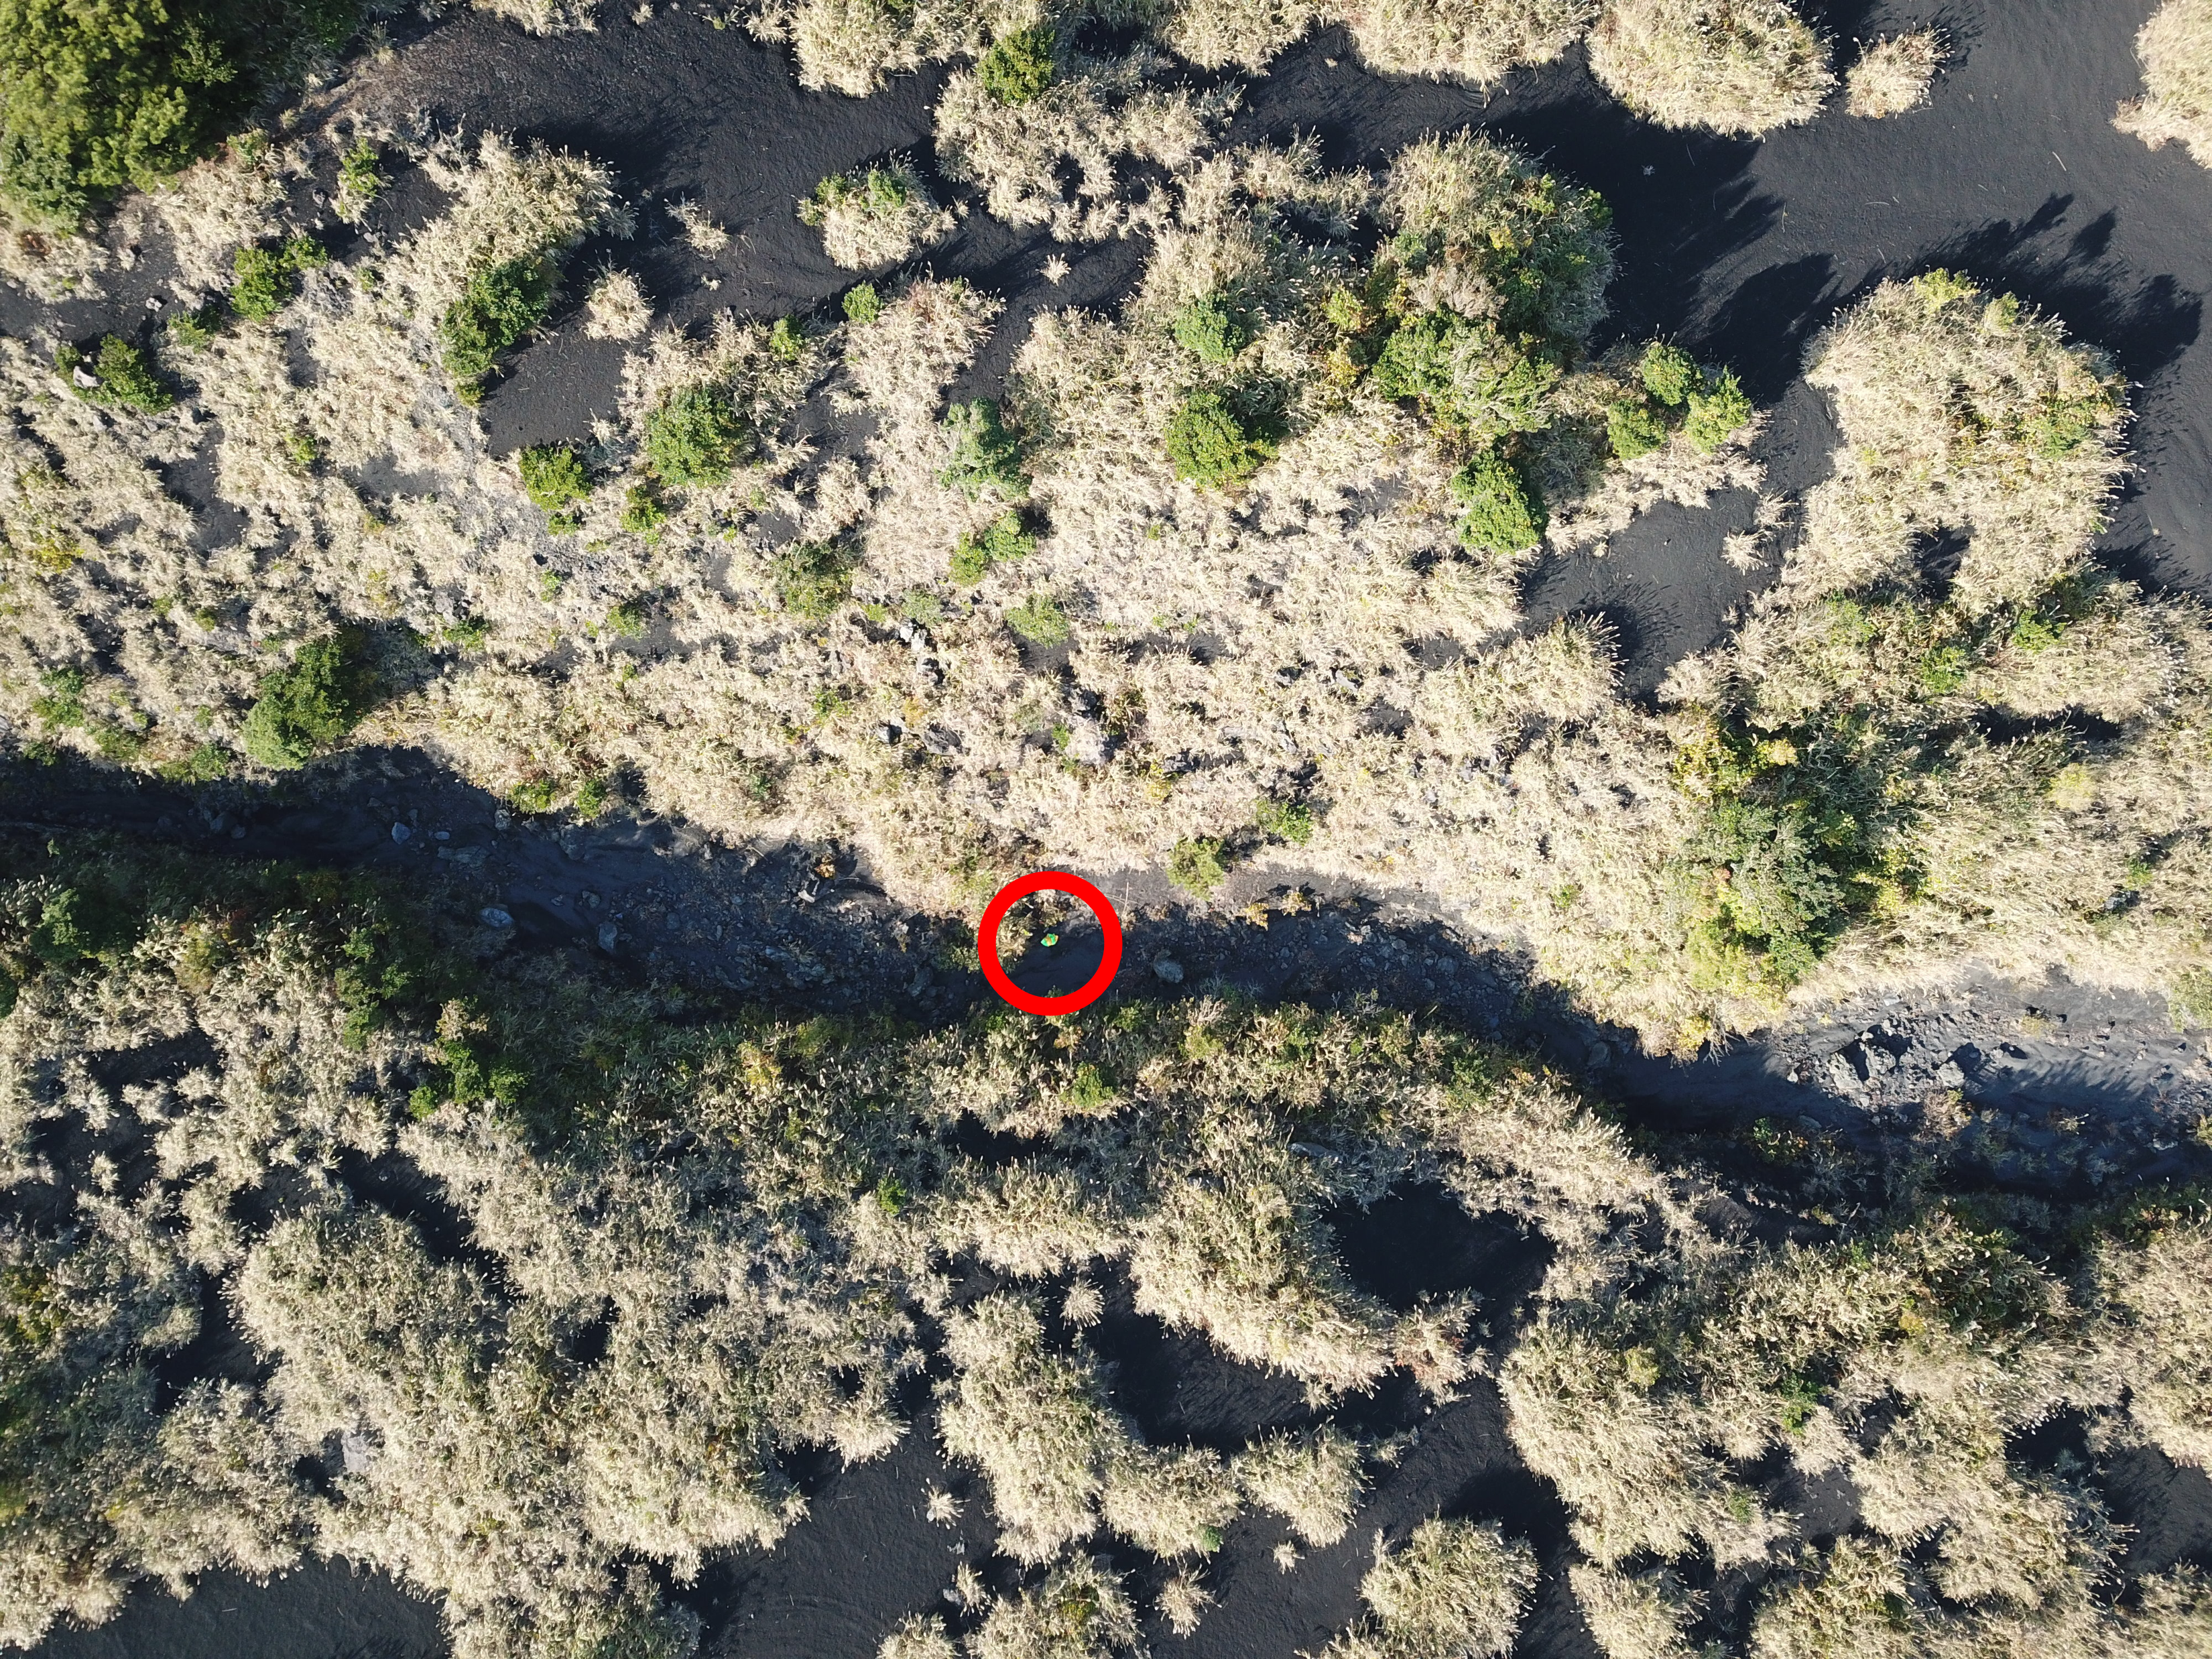
\includegraphics[width=0.8\linewidth]{pic_search/drone1.png}
    \caption{ドローンからの発見時の様子1}
    \label{fig:drone1}
\end{figure}

\begin{figure}[H]
    \centering
    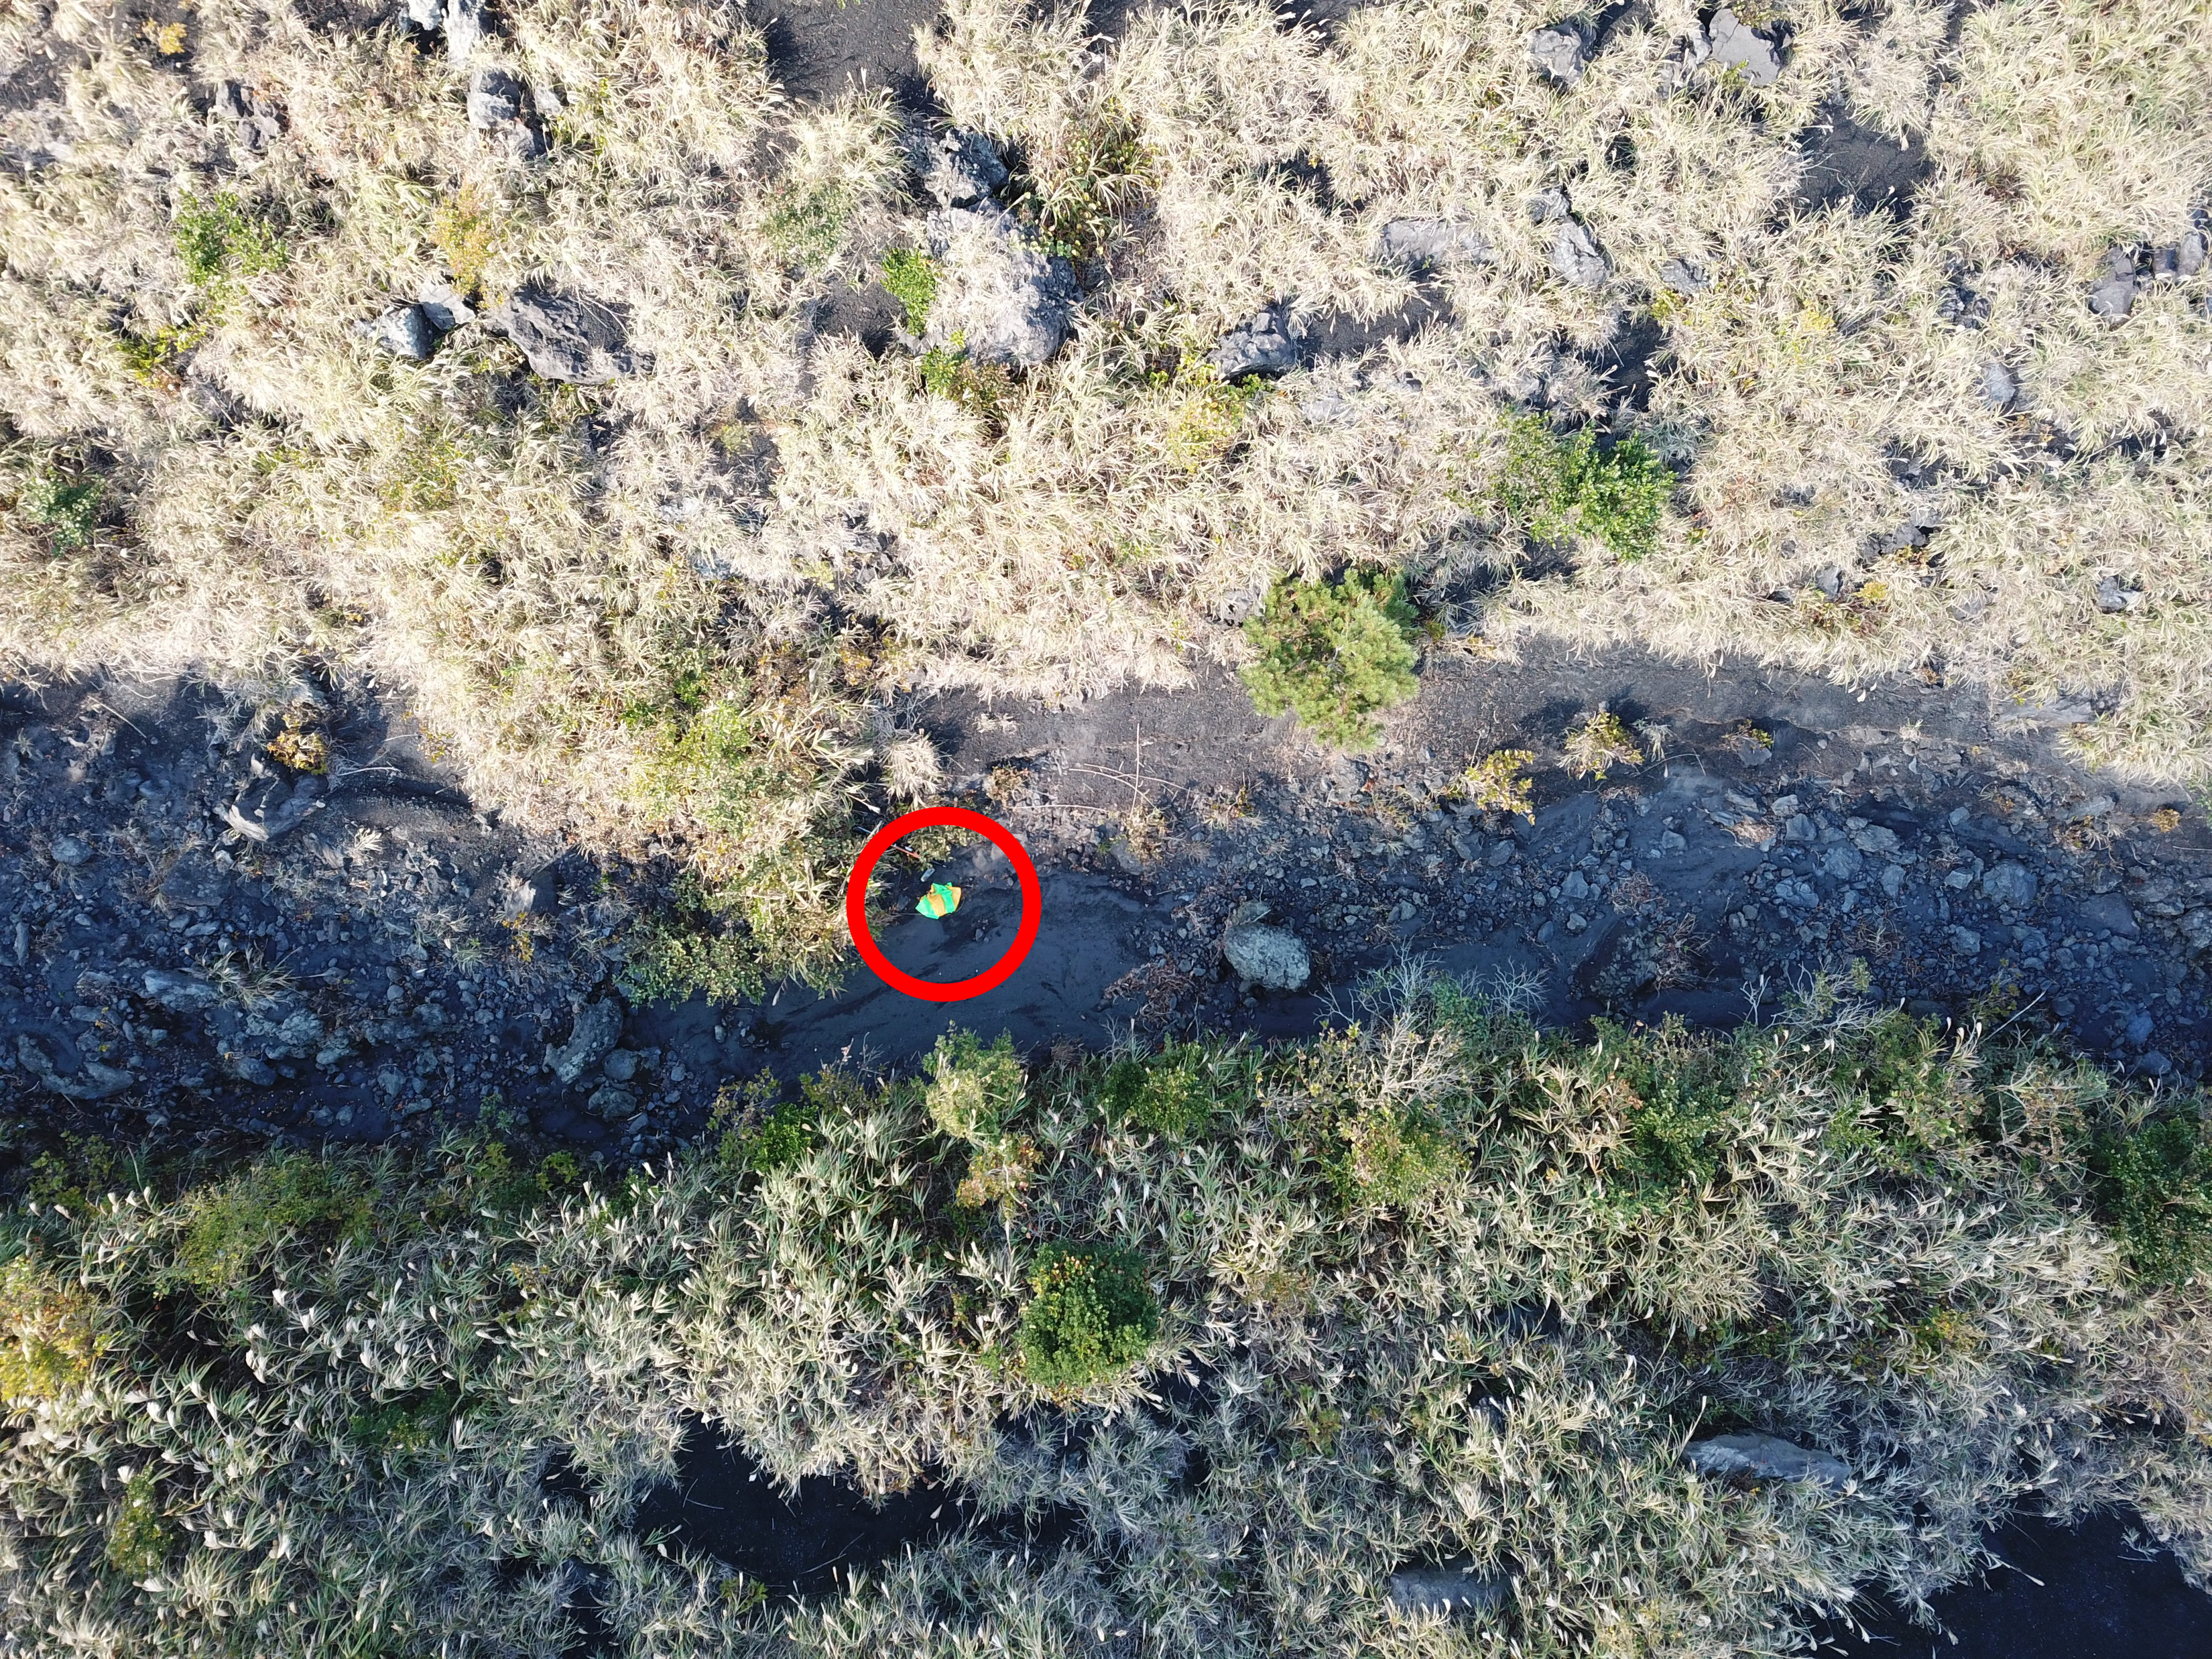
\includegraphics[width=0.8\linewidth]{pic_search/drone2.png}
    \caption{ドローンからの発見時の様子2}
    \label{fig:drone2}
\end{figure}

\subsection{反省事項}
\begin{itemize}
    \item 捜索隊2つ目をすぐに向かわせなかった。\\
    捜索隊を多く向かわせる必要があったが、指揮者が早急に指示を出さなかった。
    次回からは出せる限りの捜索隊を迅速に向かわせる。
    \item 捜索隊が2つが効率良く探せなかった。\\
    指揮者が推定落下地点についた2隊に具体的な指示を与えなかった。
    その結果手当たり次第探すだけでむらが生じてしまった。
    今後は、第1隊は落下推定地点の北側、第2隊は南側を捜索する等指示するようにする。
\end{itemize}

\section{位置推定ソフトの開発について}
本打上実験では機体からのGPSが開傘後の上空\SI{100}{m}時点で途絶しており、GPSの最終値は実際の機体落下位置とは異なる座標を示していた。
さらに、防犯ブザーも機能せず、機体の位置把握がドローン以外ではほぼ不可能な状況であった。
そのため、指差しでの機体落下位置推定技術の重要性を再認識し、落下位置の誤差範囲なども考慮して機体落下位置を指差しから推定する位置推定ソフトの開発に着手した。

\subsection{指差しによる機体落下位置推定の概要}
CREATEでは、GPSデータが取得できない状況における機体捜索での機体発見確率を上昇させるために、指差しによる機体落下位置推定を行っている。
本節では指差しによる機体捜索推定の概要について説明する。

また、指差しによる誤差には以下の数種類がある:
\begin{itemize}
    \item 機体が丘などで隠れてしまい、落下直前まで目視で確認することができないことによる誤差
    \item 指で落下方向を決定することの限界による、機体落下方向と指差し方向がずれていることによる誤差
    \item 観測者の位置を決定するGPSの精度(本打上実験では半径\SI{4}{m}の精度)が悪いことによる観測者の位置の誤差
    \item 直線を決定するときに発生する誤差
\end{itemize}
ここで、各誤差の寄与を考える。本打上実験を例にすると、機体は射点から直線距離で約\SI{380}{m}先に落下した。
まず、正確な機体落下位置から角度$\theta = \SI{1}{\deg}$だけ異なる方向の直線を引いてしまったとする。
このとき、射点からの距離$r=\SI{380}{m}$付近における直線上の位置と機体落下位置との差は
\begin{equation}
    r\times\frac{\pi\theta}{180} \approx \SI{6.6}{m}
\end{equation}
となる。すなわち、GPSの精度が悪いことによって直線が平行移動する誤差に比べて、
角度が異なることの誤差の寄与の方が十分に大きい。
\footnote{同一の端末で異なる位置のGPSを取得した場合、その間のGPSの誤差の揺らぎは考慮しなくてよい。
したがって、誤ったGPSを用いた直線は正しいGPSを用いた直線を平行移動させたものとなる。}
そのため、以下では作成する直線と真の機体落下位置方角のずれについて考察する。
なお、ここでは理想的な状況として、機体は十分に低い高度において観測できているとする。

まず、機体の落下位置が確認できた場合において、指で落下方向を決定することの限界による誤差については
最大でも\SI{4}{\deg}程度(機体落下位置付近において\SI{18}{m}程度の誤差)と見積もる。
次に、直線を決定するときに発生する誤差について考察する。現段階においては、直線を作成する方法については2種類あると考えている:
\begin{itemize}
    \item 観測者の指が示す方角へ距離$d\,\si{m}$だけ離れた場所の座標をGPSで取得し、2点を通る直線を作成する。
    \item 観測者の指が示す方角をコンパスで測定し、観測者の座標とその方角から直線を作成する。
\end{itemize}
CREATEの慣習により現在では2点を通る直線を作成しているが、$d$が小さいときに誤差が大きくなることや、
GPSを2点で取得しないといけない問題などがあり、精度については疑問が生じている。
そのため、コンパスを用いる方法との比較を行うことが今後の課題である。

以下ではコンパスで測定する方法の誤差について考察する。
コンパスで測定した方角を真の方角に修正するためには磁気偏角の値が必要である。
磁気偏角の値は国土地理院の磁気図(\url{https://www.gsi.go.jp/buturisokuchi/menu03_magnetic_chart.html}\red{あとでbibtex作るの忘れないこと。})から取得している。
磁気図を参照すると、\SI{0.5}{\deg}程度の分解能でプロットされているため、磁気偏角の誤差は最大で\SI{0.5}{\deg}と見積もれる。

さらに、コンパスが指す北と磁北のズレである自差についても考慮する必要があるが、磁気センサが内蔵されているスマートフォンのコンパスアプリを用いることで考慮しなくて良いと考えられる。
スマートフォンの地磁気センサは簡単にキャリブレーションを行うことができるため、周囲の磁性体の影響を受けにくいからである。以上より、コンパスを用いて直線を決定する方法では、
真の方角から\SI{5}{\deg}のずれに収まると考えられる。
したがって、GPSを取得することができなくとも\qtyproduct[product-units = bracket-power]{35 x 35}{\metre}の範囲を捜索すれば機体が見つかる可能性が高い。
以上より、指差しによる機体落下位置推定はアナログではあるものの有効だと考えている。

\subsection{位置推定ソフトに必要な機能}
位置推定ソフトに必要な機能について列挙する:
\begin{enumerate}
    \item 指差しをしている人の座標と方向から機体落下位置方向の直線を作成する。
    \item 生じる誤差を考慮して、機体落下可能性が高い範囲を決定する。
    \item 受信できたGPSデータから、機体の飛行経路をプロットする。
\end{enumerate}
これらを同一マップ上に示すことができれば効率的に捜索を行うことができ、機体発見可能性が上昇すると考えた。

\subsection{現段階の開発進捗と今後の展望}


\end{document}